\begin{figure}[H]
    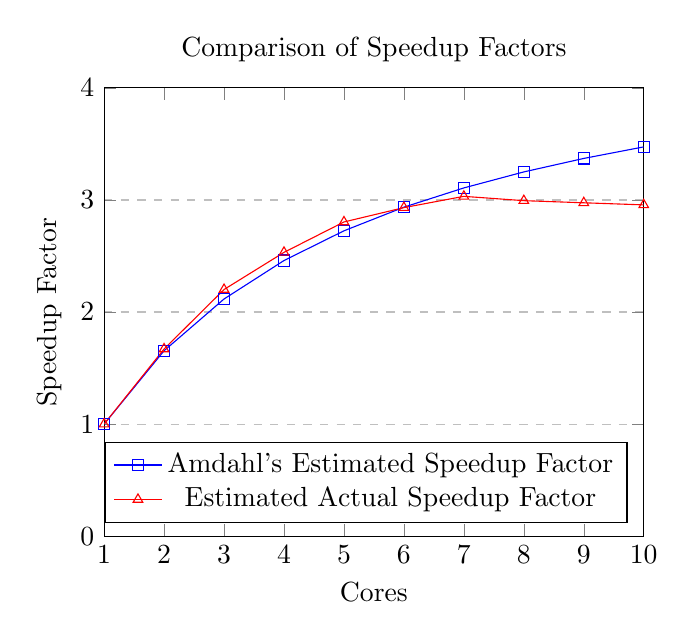
\begin{tikzpicture}
    \begin{axis}[
        title={Comparison of Speedup Factors},
        xlabel={Cores},
        ylabel={Speedup Factor},
        xmin=1, xmax=10,
        ymin=0, ymax=4,
        xtick={1,2,3,4,5,6,7,8,9,10},
        ytick={0,1,2,3,4},
        legend pos=south east,
        ymajorgrids=true,
        grid style=dashed,
    ]
    
    \addplot[
        color=blue,
        mark=square,
        ]
        coordinates {
        (1,1)(2,1.6545667448)(3,2.1163255118)(4,2.4595300263)(5,2.7246432706)(6,2.9355955681)(7,3.1074458061)(8,3.2501437611)(9,3.3705274321)(10,3.4734513278)
        };
        \addlegendentry{Amdahl's Estimated Speedup Factor}
    
    \addplot[
        color=red,
        mark=triangle,
        ]
        coordinates {
        (1,1)(2,1.6702127660)(3,2.2009345794)(4,2.5322580645)(5,2.8035714286)(6,2.9315352697)(7,3.0321888412)(8,2.9936440678)(9,2.9747368421)(10,2.9560669456)
        };
        \addlegendentry{Estimated Actual Speedup Factor}
    
    \end{axis}
    \end{tikzpicture}
    \caption{A comparison on the estimated speedup factor from Amdahl's law, Gustafson's law and the actual Speedup factor for 3DM on DUT 2}
\end{figure}
